\chapter{Object Detection}
\label{chapter:object-detection}

Object Detection is a field of \acf{cv} whose objectives are to classify and locate objects on an image. Contrary to Object Recognition, whose sole goal is to identify which objects are present on a given image, object detection not only classifies the objects, but also outputs a bounding box and its position on the image. 

Using previous calibration and sensor fusion methods, detailed in chapter~\ref{chapter:calibration} and~\ref{chapter:sensor-fusion}, respectively, this chapter intends to add to the previous work, allowing the segmentation of \acfp{roi} on the point cloud. Those \acp{roi} correspond to objects detected by the image, using the camera as the input and not the \ac{lidar}, since the point cloud obtained is expected to be interfered by other \acp{lidar}.

To succesfully detect \acp{roi} in a given image and estimate the corresponding point-cloud for that region, three tasks are required: 
\begin{enumerate}
	\item Perform object detection on the camera image feed, computing the bounding boxes that delimite the \acp{roi};
	\item Select the objects' of interest bounding boxes from the pool of detected objects;
	\item Filter the point cloud on the \acp{roi} using the image bounding boxes information.
\end{enumerate}

\section{Object Detection on Image}
\label{sec:object-detection:image}

Object Detection on image is normally achieved with \acfp{cnn}, as detailed in Section~\ref{sec:sota:object-detection}, using deep learning tecnhiques to train the \acl{nn}. From the available \acp{cnn} frameworks and \acl{sota} solutions, the author choose \ac{yolo}, due to its accuracy, real-time object detection capabilities and low resource usage\footnote{On this context, low resource usage is considered in comparison with other available solutions with similar detection accuracy. See a detailed comparison on~\cite{Redmon2018}.}~\cite{Redmon2016, Redmon2017}

Pre-trained models are available for \ac{yolo}v2 and \ac{yolo}v3, using the \ac{pascal-voc} and \ac{coco}'s dataset.As detailed in Section~\ref{sec:sota:object-detection} and on~\cite{Redmon2018}, \ac{yolo}v3 surpasses its prior versions, therefore only the latter version will be used. 

For all 3 versions of \ac{yolo}, a ``tiny'' counterpart is also available. The ``tiny'' \ac{yolo} versions consist of a smaller network that can perform faster classification at the expense of detection accuracy (bounding box position, dimensions and object class). For the scope of this research, we are interested on having a very good estimation of the bounding boxes dimensions and position, since those will be used to detect the corresponding \acp{roi} on the point cloud. 

\subsection{Setup Specifications}
To summarize the stated above, our image object detection uses the ac{yolo}v3 \ac{cnn}, with pre-trained weights for the \ac{coco} image dataset, running on the Redmon's \texttt{Darknet} framework wrapped in a multi-threaded \ac{ros} node. Darknet is compiled with \ac{cuda} and \ac{opencv} enabled, for \ac{gpu} accelaration and native visualization of the classified images with bounding boxes.

The image objection detection is performed on a standart laptop with a Intel\cp~i7 \ac{cpu} and a Nvidia\cp~GeForce GT 740M. Their relevant specifications are given on table~\ref{tab:computer-specs}, along with information about the graphics card driver and \ac{cuda} version used.

\begin{table}[H]
	\renewcommand{\arraystretch}{1.2}
	\centering
	\begin{tabular}{@{}lp{7cm}l@{}}
		\toprule
		\multicolumn{2}{l}{Specification} & Value \\ \midrule
		\multicolumn{2}{l}{\emph{\ac{cpu}}} & \\
		\phantom{a} & Model   & Intel\cp~Core\texttrademark~i7-4700MQ \\
								& Maximum clock frequency & \SI{2.40}{\giga\hertz} \\
								& Number of cores & 4 \\ 
		\midrule
		\multicolumn{2}{l}{\emph{Graphic Card}} & \\
		\phantom{a} & Model   & Nvidia GeForce GT 740M \\
								& Maximum \ac{gpu} clock frequency & \SI{1058}{\mega\hertz} \\
								&	Maximym memory transfer rate & \SI{1840}{\mega\hertz} \\
								&	Nvidia driver number & 418.87.01 \\
								& Total memory size & \SI{2048}{\mega\byte} \\
								& Bus width & \SI{64}{\bytes} \\
								& Theorerical Floating Point Operations & \SI{250.9}{\giga\flops} \\
		\midrule 
		\multicolumn{2}{l}{\emph{\ac{cuda}\texttrademark}} \\
								&	Version & 10.1 \\
								&	Dedicated memory size available on \ac{gpu}& \SI{2004}{\mega\byte} \\
								& Available \ac{cuda} cores on \ac{gpu} & 384 \\
		\bottomrule
	\end{tabular}
	\caption{Relevant specifications for \ac{cpu}, graphics card, \ac{cuda} and Nvidia\texttrademark driver.}
	\label{tab:computer-specs}
\end{table}


\subsection{Integration with \ac{ros}}
\texttt{Darknet} (the \ac{nn} framework underlying \ac{yolo}) integrates with \ac{ros} using an Open-Source package developed by Marko Bjelonic~\cite{MarkoBjelonic}, \texttt{darknet-ros}. This package runs the Redmon's \texttt{Darknet} framework and wraps its configuration, input images and outputs results on a \ac{ros} node, containing an action server and several topics messages.

To operate \texttt{darknet-ros}, a \ac{ros} launch file is used. This launch file specifies the network model, configuration, weights and other \ac{ros} parameters, and is adapted from \texttt{darknet-ros} package launch file~\cite{MarkoBjelonic}. 

For image object detection, \texttt{darknet-ros} is used as a standalone node, with its input images being provided by a \texttt{rosbag} player, playing either the \ac{kitti} dataset data or the experimental setup. An \ac{opencv} image visualization window is embedded natively in \texttt{Darknet}, if it is compiled alongside it, and is used to visualize the classified images with bounding boxes.


\subsection{Results}
It is out the scope of this thesis to analyze or develop image object detection methods. Image object detection is used on this thesis as ``means to an end'': detecting \acp{roi} on image to compute their corresponding point cloud. Therefore,  exhaustive tests comparing the \ac{yolo} performance under different thresholds, lightning conditions and images were not carried. Instead, qualititative assesments were performed to estimate a good threshold for confindence detection that maximizes the number of detected objects.

\texttt{Darknet} is set with a default confidence threshold of 25\%~\cite{Redmon2016}. However, from our findings, a threshold of 30\% produces a better tradeoff between the number of detected objects and the bouding box accuracy, reason why it was choosen.

With the relevant computer specifications present on table~\ref{tab:computer-specs}, the previous described method is able to classify images with 1.1 to 1.8 \ac{fps}, depending on the dataset. Therefore, to ensure that the classification does not create a bottleneck on the system and messages are being dropped by \texttt{darknet-ros} node, the \texttt{rosbag} player is throttled.

Images are published at $\approx\SI{10}{\hertz}$ on the \ac{kitti} dataset and at \SIrange[range-units=single]{4}{8}{\hertz}. Therefore, if the we throttle the rate of \ac{ros} messages publishing to $10\%$ of the original rate, messages are published at a maximum of \SI{1}{\hertz}, which ensures that no image frame dropping happens on \texttt{darknet-ros} node.

Exemplary results are presented below, either for the \ac{kitti} dataset and experimental data recorded. 
	
\subsubsection{\ac{kitti} Dataset}
Exemplary results of the object detection method applied to the \ac{kitti} dataset are presented on figure~\ref{fig:kitti-object-detection}. 

With the relevant computer specifications present on table~\ref{tab:computer-specs}, the previous described method is able to classify images at 1.3 to 1.8 \ac{fps}. Exemplary results are presented below, either for the \ac{kitti} dataset and experimental data recorded. 

\begin{figure}[ht!]
	\centering
	\begin{subfigure}[c]{0.8\textwidth}
		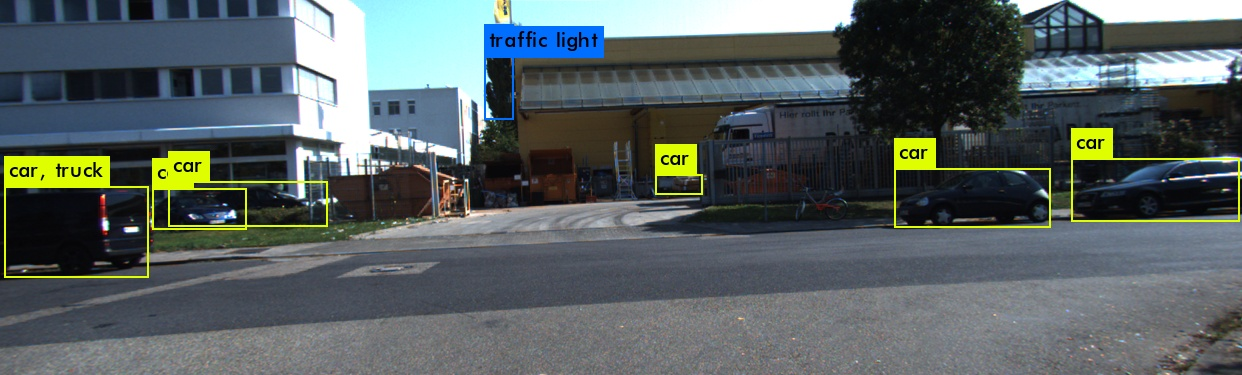
\includegraphics[width=\textwidth]{img/object-detection/kitti-4.jpg}
		\caption{Object detection on an urban area. Classification and bounding box dimensions and position are accucarate, with exception of the traffic light bounding box, that is mistaken with a tree top.}
		\label{fig:kitti-yolo-3}
	\end{subfigure}
	\\ \vspace{4mm}
	\begin{subfigure}[c]{0.8\textwidth}
		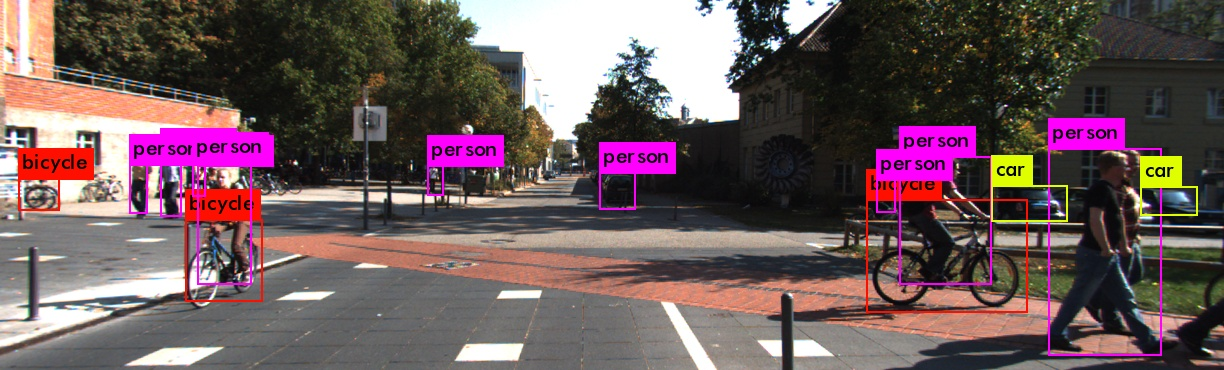
\includegraphics[width=\textwidth]{img/object-detection/kitti-2.jpg}
		\caption{Object detection on Karlsruhe Institute of Technology \textit{campus}. There are two detection errors on this image. On the center, two road poles and a car are labelled as a person. On the left, two persons are grouped togther in one bounding box.}
		\label{fig:kitti-yolo-2}
	\end{subfigure}
	\caption{Object detection results for the \ac{kitti} dataset, using \ac{yolo}v3 with a confidence threshold of 30\%, trained for the \ac{coco}'s image dataset. With the specifications present on table~\ref{tab:computer-specs}, a 1.3 to 1.8 \ac{fps} were registered when classifying the images.}
	\label{fig:kitti-object-detection}
\end{figure}


\subsubsection{Experimental Data acquired}
Exemplary results of the object detection method applied to the experimental data gathered on a \ac{msl} robotic football field, at \acf{irislab}, are presented on figure~\ref{fig:experimental-object-detection}. The confidence threshold of \ac{yolo} is set to 30\% and with the specifications present on table~\ref{tab:computer-specs}, a 1.1 to 1.4 \ac{fps} were registered when classifying the images.

Since experimental data was stored on raw format, as detailed on Section~\ref{sec:calibration:extrinsic}, de-Bayering and conversion to RGB of the raw image must be performed using the \texttt{image\_proc} package before feeding the data to the \texttt{Darknet}.

\begin{figure}[ht]
	\centering
	\begin{subfigure}[t]{0.45\textwidth}
		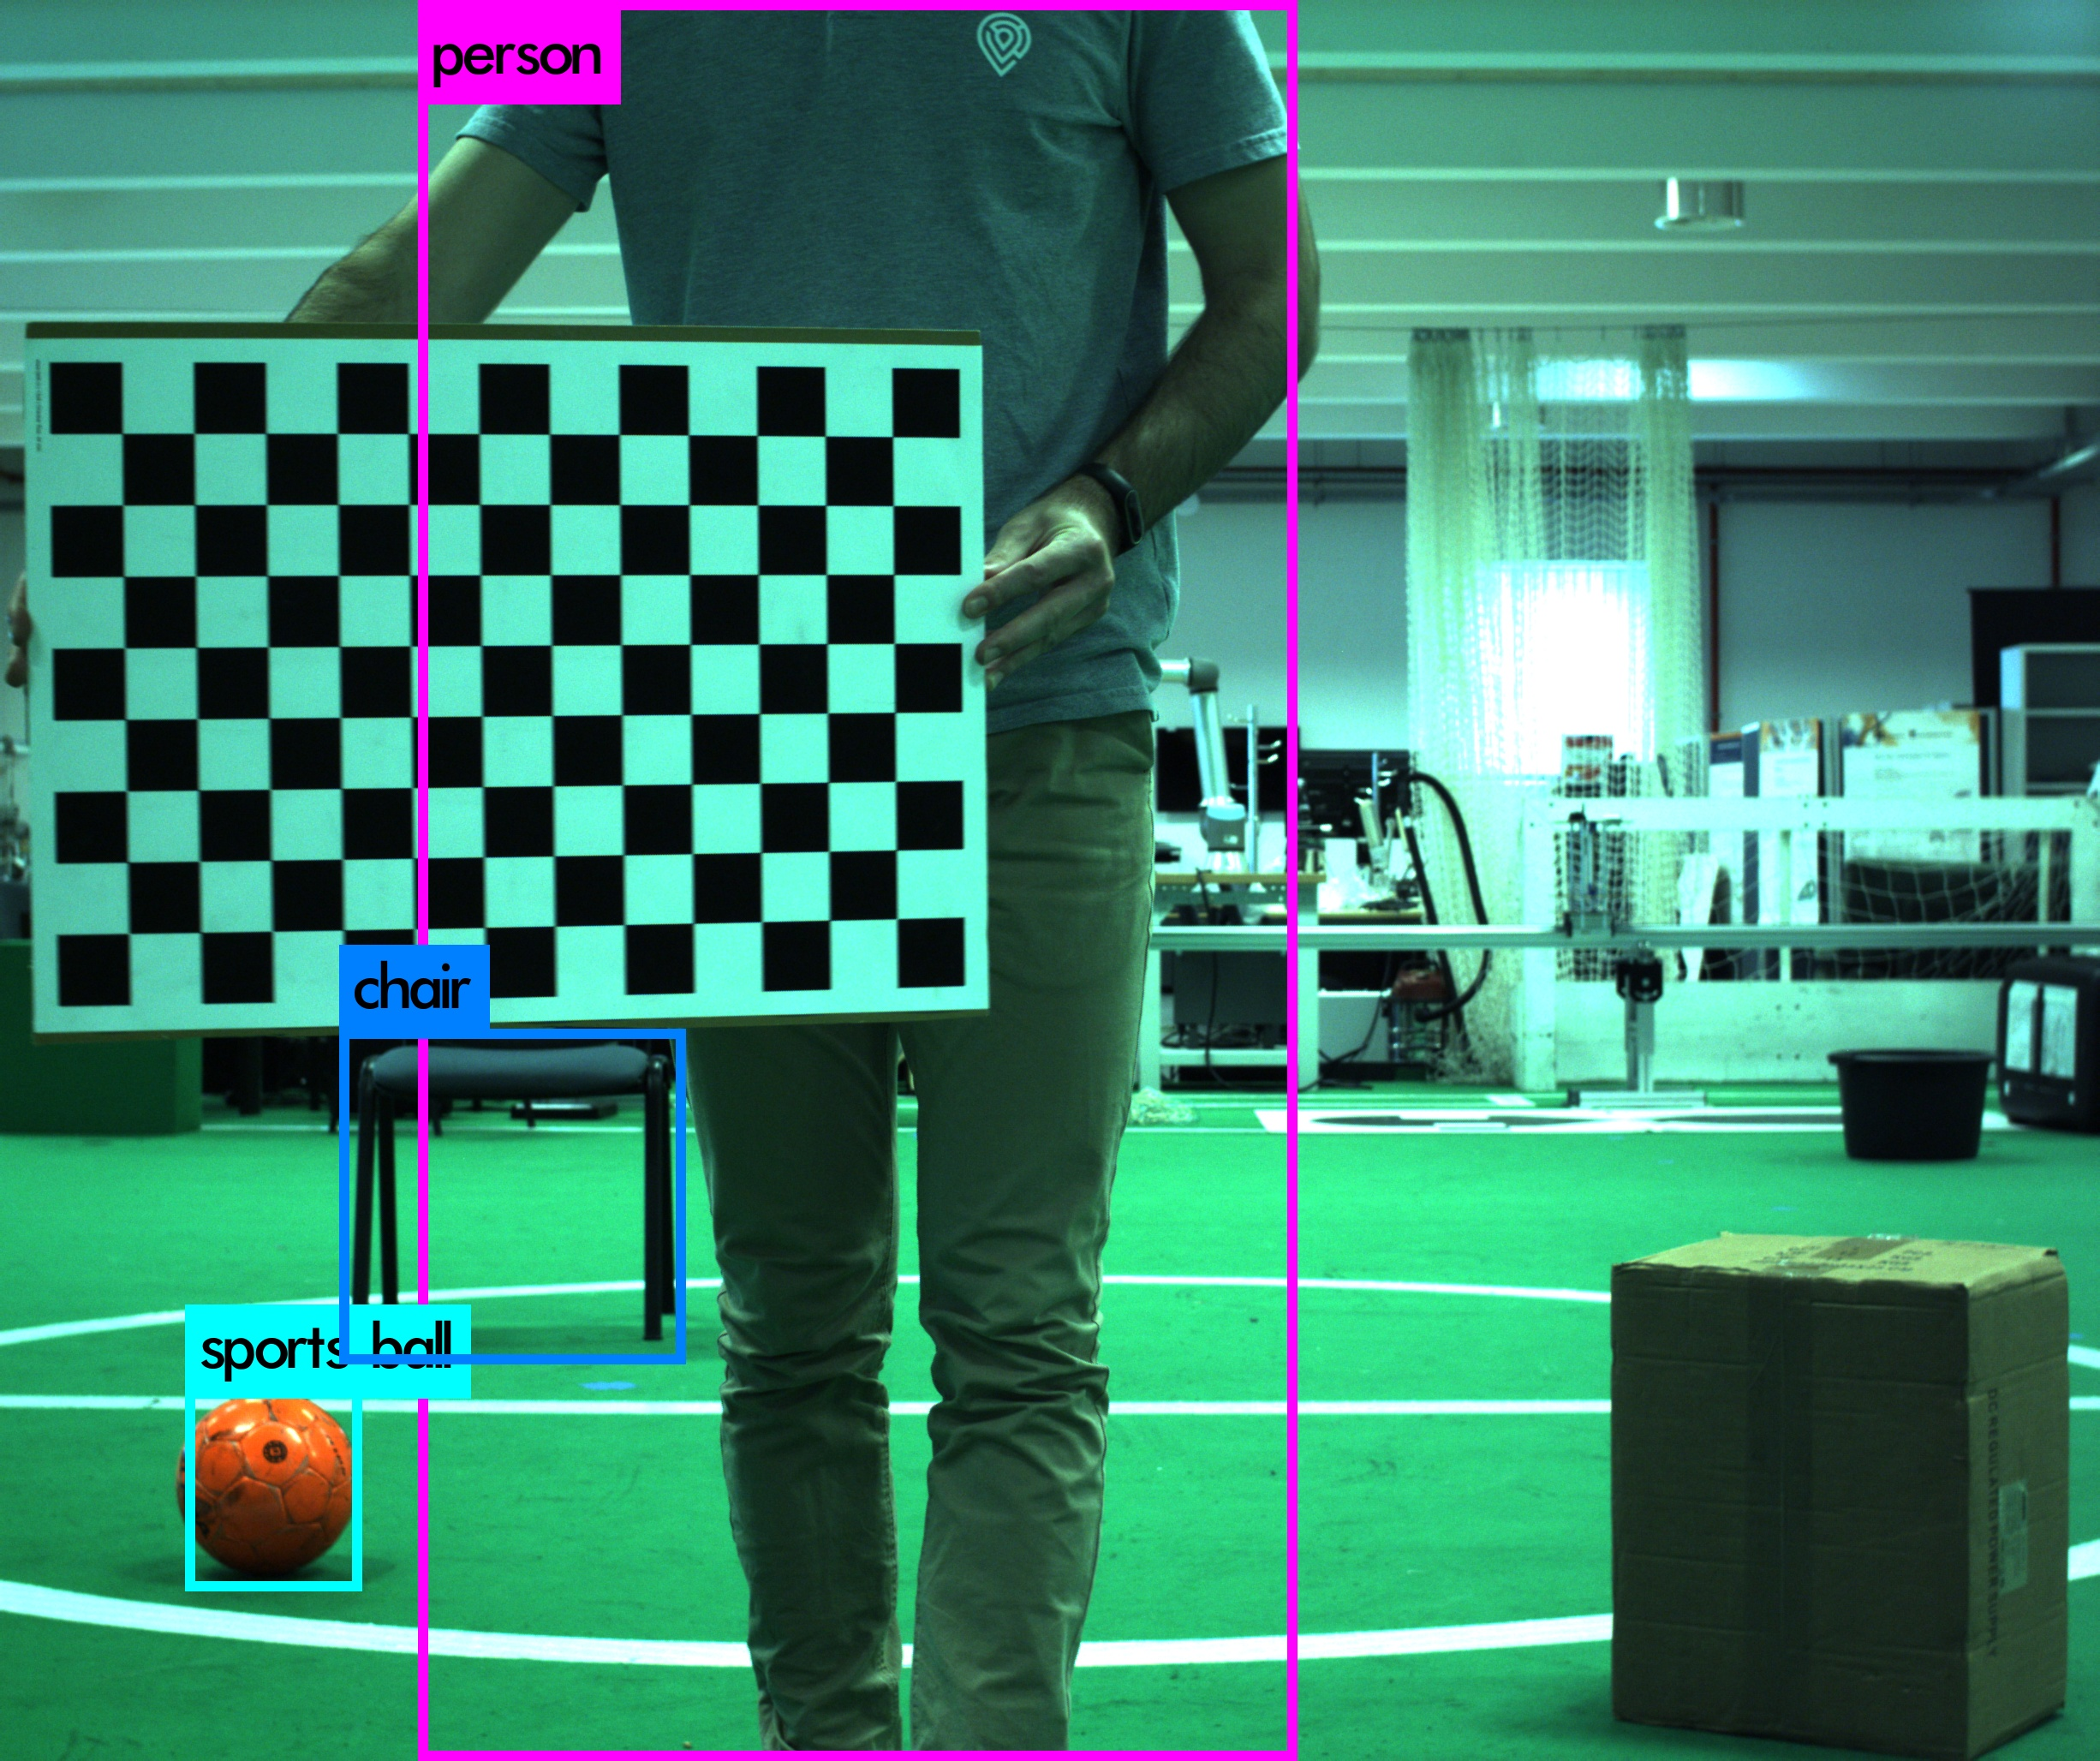
\includegraphics[width=\textwidth]{img/object-detection/experimental-1.jpg}
		\caption{Object detection on a \ac{msl} football field, at \ac{irislab} research facility. Despite the occlusion of the chair and person, \ac{yolo} is capable of recognizing them both.}
		\label{fig:experimental-yolo-1}
	\end{subfigure}
	\qquad
	\begin{subfigure}[t]{0.45\textwidth}
		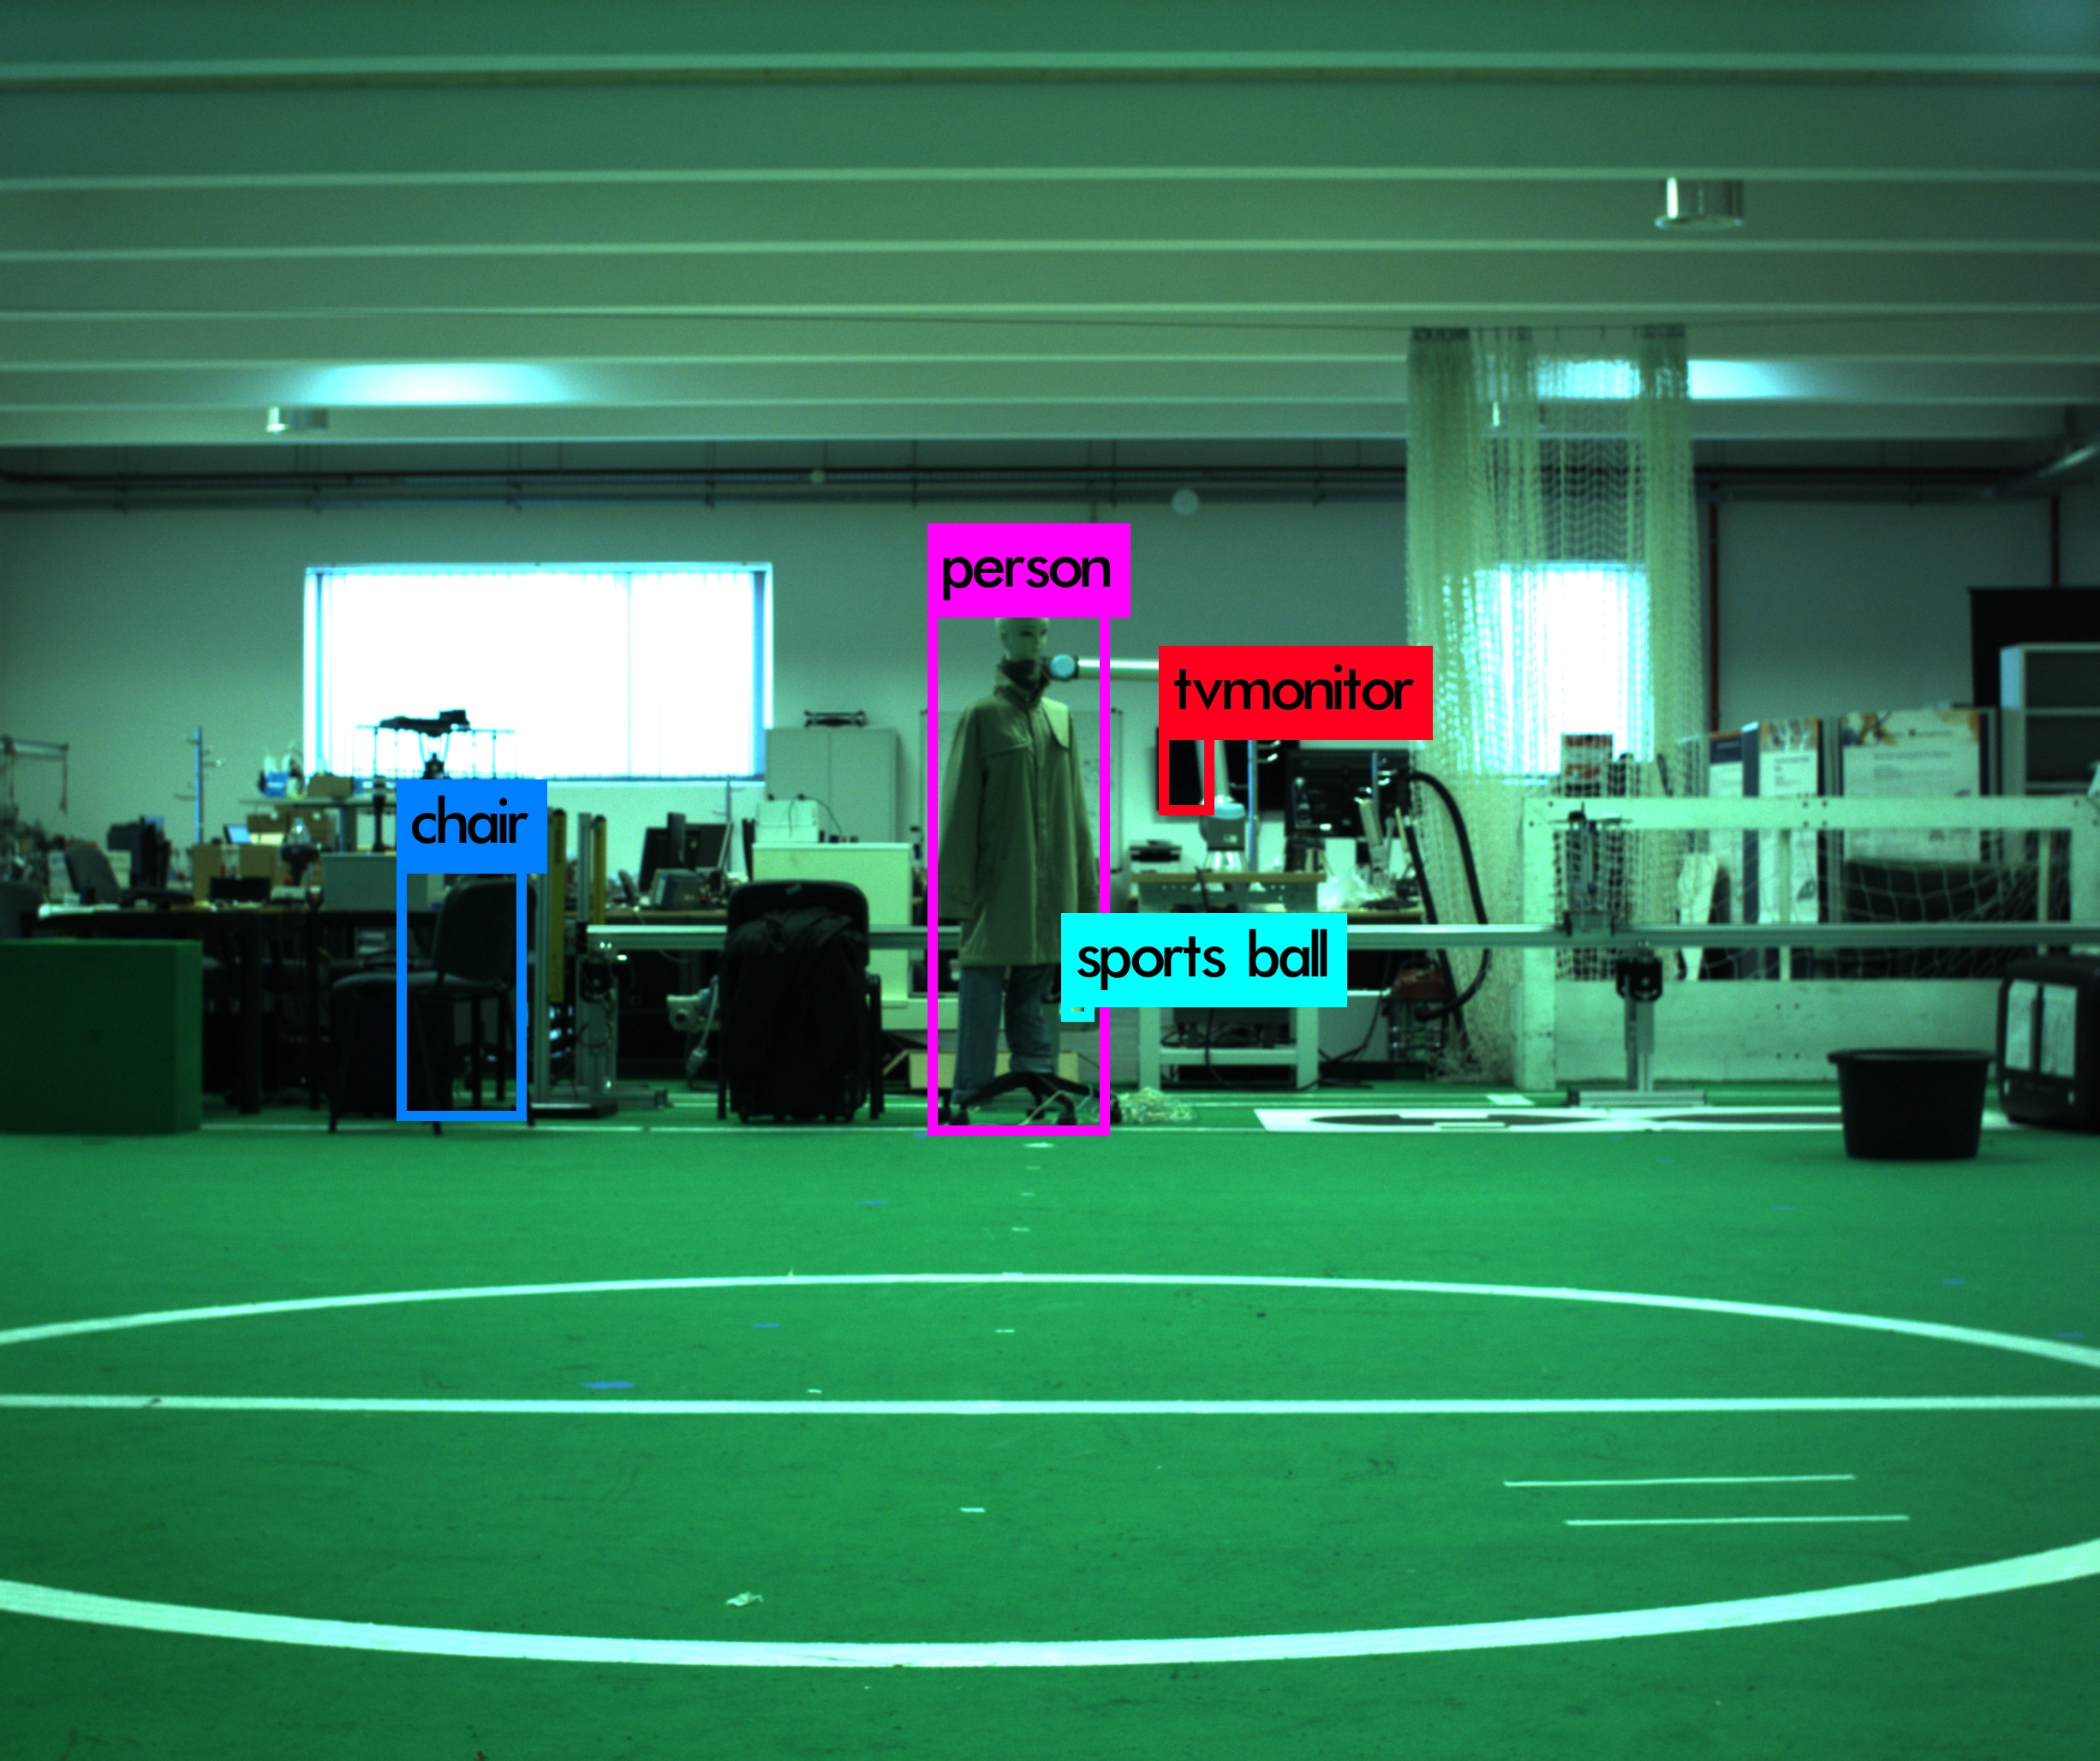
\includegraphics[width=\textwidth]{img/object-detection/experimental-2.jpg}
		\caption{Object detection on a \ac{msl} football field, at \ac{irislab} research facility.  It detect the human dummy as a person and confunses its hands for a sports ball. On the back, the tv monitor is correctly classified, but the bouding box is smaller, since it is occluded by the robotic arm.}
		\label{fig:experimental-yolo-2}
	\end{subfigure}
	\caption{Object detection results for the experimental data gathered on a \ac{msl} robotic football field, at \ac{irislab}. \ac{yolo}v3 is used with a confidence threshold of 30\% and trained for the \ac{coco}'s image dataset. With the specifications present on table~\ref{tab:computer-specs}, a 1.1 to 1.4 \ac{fps} were registered when classifying the images. Note that since the data was stored on a raw format, deBayrization and rectification needs to be performed by \texttt{image\_proc} node before the RGB images being feed to the \texttt{Darknet}.}
	\label{fig:experimental-object-detection}
\end{figure}


\section{Correspondences between objects on image and point-cloud}
A calibrated camera and \ac{lidar} setup, on which both are calibrated intrinsically and their rigid body transform is known\footnote{The method used to determine this rigid body transform on our experimental dataset is outlied on Section~\ref{sec:calibration:extrinsic}. Chapter~\ref{chapter:calibration} details all the calibration procedures that are pre-required for this section. For \ac{kitti} dataset, suchs transformations are already given.}, data conversion between the two coordinate frames is possible, as shown previously on chapter~\ref{chapter:sensor-fusion}. 

Matching the camera's \acp{roi} with \ac{lidar}'s requires converting the data to a common coordinate frame between the two sensors and then using a matching algorithm to select the point cloud points that correspond to the classified object on the image. Selecting the \acp{roi} on the point cloud that correspond to the image objects bounding boxes implies establishing a $2D \leftrightarrow 3D$ correspondance between the data. Two alternatives are possible, similar to those presented on Chapter~\ref{chapter:sensor-fusion}. The first one consists on converting the 2D pixels to a 3D ray referenced on the \ac{lidar} coordinate frame, throug ray-casting; and the second one consists on projecting the 3D points registered by the \ac{lidar} to the the image pixels. After ``converting'' a two-dimensional \acp{roi} to a tridimensional \acp{roi}, aA tridimensional bounding box can be estimated and drawn, for visualization purposes, on the point cloud. 

This section explains the method implemented for computing the point cloud bounding boxes, by using the information of the image bounding boxes obtained using \ac{yolo}, as detailed on Section~\ref{sec:object-detection:image}. Two matching algorithms are presented, along with their results and a brief comparison. Bouding box estimation is also detailed, along with results for every stage of the processing chain.


\subsection{\texttt{darknet-ros} Package Limitations and Contributions}
\texttt{Darknet-ros} encapsulates the \texttt{Darknet} framework and allows its connection with other nodes on the \ac{ros} network. Excluding its interface for \ac{nn} configuration (\ac{nn} model and weigths) and data input topics, which are detailed on~\cite{MarkoBjelonic}, \texttt{darknet-ros} provides 3 output topics:

\begin{enumerate}
	\item \texttt{found\_object}: a standard integer message that indicates the number of objects found by the \texttt{Darknet} framework when running the desired \ac{nn} model;
	\item \texttt{detection\_image}: A \ac{ros} image topic, similar to its input, but with the detection bounding boxes drawn;
	\item \texttt{bboxes}: a custom message topic that contains an header with metadata and an array of bounding boxes detected on the image. Each bouding box element of this array indicate its class, id, probability and the minimum and maximum points that define the bounding box for that object;
\end{enumerate}

To the purpose of this work, precise synchronization between the point cloud and \texttt{darknet} outputs is required. However, \texttt{darknet-ros} does not provide an interface with this in mind, lacking information for synchronizing the \texttt{found\_objects} topic with the other topics.

Therefore, \texttt{darknet-ros} package was improved to mitigate this problem. Our proposal consists on defining a custom message for \texttt{found\_objects} topic that additionatly to the standard integer indicating the number of objects found, also contains an header with the time stamps and frame id for synchronization. \texttt{darknet-ros} code was changed in order to publish this new message type under \texttt{found\_objects} topic, ensuring also  backwards compatitibility.

Those changes were later submitted to the original author of \texttt{darknet-ros}, which were accepted and merged with the publicly available source code~\cite{MarkoBjelonic}.


\subsection{Ray Casting}
The first implemented algorithm to match image and point cloud \acp{roi} envolves a technique of ray casting, i.e., casting a ray from the camera center that passes throught the desired pixel, projecting it from the two-dimensional image representation to a three-dimensional suited for comparing with it \ac{lidar} data.

After data convertion from one coordinate frame to the other, using the rigid body transform determined on Section~\ref{sec:calibratiuon:extrinsic}, ray-casting allows the determination of 4 lines that delimite a 3D section of the point cloud, by casting the corners of the image bouding box. These 4 lines, transformed to the \ac{lidar} coordinate frame, define the boundaries of an infinite rectangular pyramid. Considering a near and far limit parallel cut planes, that are  perpendicular to the pyramid orientation, a pyramidal frustum is obtained (see figure~\ref{fig:pyramid-frustum}), containing all the point cloud points that are part of the tridimensional \ac{roi} for the object detected.  

However, since the bouding box on the image contains more than the object that is recognized, the point cloud region will also contain outliers, i.e., points that are present in the \ac{roi} but are not part of the object of interest.

\begin{figure}[H]
	\centering
	\def\svgwidth{0.3\columnwidth}
	\graphicspath{{img/image-object-to-point-cloud/}}
		\includesvg{img/image-object-to-point-cloud/pyramid-frustum}
	\caption{Pyramid Frustum. The gray section corresponds to the pyramid frustum volume between the near and far plane on the boundaries defined by the pyramid.}
	\label{fig:pyramid-frustum}
\end{figure}

Back-projection the pixels to 3D rays to define the boundaries of the point cloud is not sufficient for a proper frustum filtering. To segment a frustum out of the \ac{lidar} point cloud, we are required to determine:
\begin{itemize}
	\item The pure rotation coefficients that aligns the \ac{lidar} coordinate frame to a new frame, oriented to the \ac{roi};
	\item The vertical and horizontal \acf{fov} of the pyramid frustum;
	\item The near and far cut planes limits.
\end{itemize}

\subsubsection{Back Projection}
Projecting pixels to a ray (also called back projection) is the inverse process that is used to create an image on a camera\footnote{A camera projects the world points to a two dimensional plane. See Section~\ref{sec:sota:camera}}. The projection matrix defined in equation~\ref{eq:camera_transform_full}, if inverted, can be used to calculate the transformation matrix that  back projects pixels into rays.

Since on our implementation the transformation between different coordinate frames is done separately from the back-projection algorithm, the image pixels are already defined on the camera's coordinate frame and joint rotation and translation matrix, $\begin{bmatrix} R|t \end{bmatrix}$, are the identity and a zero column vector, respectively, and therefore do not need to be considered.

Following Hartley's and Zisserman's book~\cite{mvg_book}, our back-projection operation degenerates to computing the inverse of the intrinsic camera matrix, $K$, and multiply that inverse by the pixel coordinates referenced in affine coordinates, detailed on equaiton~\ref{eq:back-projection}. The rotation and translation to convert the rays from the camera's coordinate frame to \ac{lidar}'s are applied after the ray-casting operation.


\begin{align}
	\label{eq:back-projection}
	\begin{bmatrix}
		X \\
		Y \\
		Z
	\end{bmatrix}
	 & = K^{-1} 
	\begin{bmatrix}
		u \\
		v \\
		1
	\end{bmatrix}
\qquad \wedge \quad
	K = 
	\begin{bmatrix}
		f_x & 0 & c_x \\
		0 & f_y & c_y \\
		0 & 0 & 1.0
	\end{bmatrix}
\nonumber \\	 
	&  = 
	\begin{bmatrix}
	\frac{1}{f_x} & 0 & -\frac{c_x}{f_x} \\
	0 & \frac{1}{f_y}  & -\frac{c_y}{f_y} \\
	0 & 0 & 1.0 
	\end{bmatrix}
	\begin{bmatrix}
		u \\
		v \\
		1
	\end{bmatrix}
\end{align}

\subsubsection{Rotation from the \ac{lidar} coordinate frames to the bounding boxes' coordinate frame}
Using ray-casting, the pure rotation of the \ac{lidar} coordinate frame to the bounding boxes coordinates frames can be obtained by considering the angle between the two rays that pass between the image bounding box center and the image center. Let $B^{center}$ be the image bounding box center, which can be calculated using equation~\ref{eq:bboxes-pixel-center} and $C^{center}$ be the image center, which corresponds to the intrinsic camera parameters $c_i, \forall i \in \{x, y\}$, as denoted in equation~\ref{eq:image-pixel-center}.

\begin{equation}
	\label{eq:bboxes-pixel-center}	
B^{center} = \left(\frac{x^{\text{bounding box}}_{min} + x^{\text{bounding box}}_{max}}{2}, \frac{y^{\text{bounding box}}_{min} + y^{\text{bounding box}}_{max}}{2},\right)
\end{equation}

\begin{equation}
\label{eq:image-pixel-center}
C^{center} = (c_x, c_y)
\end{equation}

Considering that their representation in a affine space is given by $P_{affine} = \left[P | 1\right]^T, \forall P \in \{B^{center}, C^{center}\}$; and denote the ray casted by the camera origin that passes through the pixels defined by the point $B^{center}_{affine}$ and $C^{center}_{affine}$, as $\vec{b}$ and $\vec{c}$, respectively, where  $\vec{b}$ and $\vec{c}$ can be determined using equation~\ref{eq:back-projection}.

The rotation of the \ac{lidar} coordinate frame to a new frame oriented to the bounding box can then be obtained by calculating the orientation quaternion between vector $\vec{c}$ and $\vec{b}$, denoted by $q$, which is capable of projecting a line from the coordinate frame of the bounding box to the \ac{lidar} coordinate frame.

\subsubsection{Horizontal and Vertical \ac{fov}}
The horizontal and vertical \ac{fov} are determined on the image plan. First, the angle between the image center and each of the bounding box limits (upper and lower) are calculated for the two dimensions, x and y. Then, the difference between the upper and lower angles is computed to obtain the \ac{fov} on that axis.

Let $\theta^{upper limit}_i$ denote the upper limit of the image bounding box, on the generic $i$ axis, that can be replaced by $x$ and $y$, and $\theta^{lower limit}_i$ represent the lower limit on that same axis. Consider the image axis origin to be at the center of the image and the \ac{fov} of the bounding box can be defined by $\Theta^{FOV}_i$ on equation~\ref{eq:image-fov}, for that same generic axis $i$.


\begin{equation}
	\label{eq:image-fov}
	\Theta^{FOV}_i = \theta^{upper limit}_i - \theta^{lower limit}_i, \qquad \forall i \in \{x, y\}
\end{equation}

\subsubsection{Near and Far Planes}
The Near and Far Cut Planes can be defined by the data and \ac{lidar} constraints. Following the datasheet of the VLP-16~\cite{vlp16}, the \ac{lidar} used on the experimental setup, and HDL-64~\cite{VelodyneHDL64}, the \ac{lidar} used on the \ac{kitti} dataset, the Near Cut Plane can be defined to \SI{1}{\meter}, since the \acp{lidar} cannot detect smaller distances.

Due to data sparsity and visualization of the data, both on the experimental and  \ac{kitti} dataset, a Far Plane of \SI{30}{\meter} is enough to garantee that all the objects of interest on the \ac{fov} are present.

\subsubsection{Implementation}
Using the constrains and methods detailed before, a \ac{ros} node, \texttt{image\_bbox\_to\_point\_cloud\_node}, is implemented to perform frustum filtering on the point cloud using the image bounding boxes given by \texttt{darknet-ros}. The node diagram is given on figure~\ref{fig:ros-graph-frustum}, where the node \texttt{Kitti\_dataset} is a \texttt{rosbag} player and \texttt{darknet-ros} is the node described in Section~\ref{sec:object-detection:image}, responsible for image object detection. \texttt{RViz} is the \ac{ros} visualizer, that shows the transforms between the coordinate frames, the original point cloud and the frustum filtered point cloud.

\begin{figure}[H]
	\centering
	\def\svgwidth{\columnwidth}
	\graphicspath{{img/image-object-to-point-cloud/}}
	\includesvg{img/image-object-to-point-cloud/frustum}
	\caption{\ac{ros} node graph corresponding to the implementation of the Point Cloud Frustum Filter node from the image bounding boxes. }
	\label{fig:ros-graph-frustum}
\end{figure}

The node also computes the pose of each of the bounding boxes in relation to the \ac{lidar} axis, both on the \ac{lidar} referential and the frustum algorithm on \ac{pcl}. 

To implement this node, \ac{pcl} frustum filter algorithm was used, along with other utilities and Eigen was also used. Eigen is a C++ library for linear algebra, matrix and vector operations and geometrical transformations, among other features~\cite{Eigenv3}.

Several variations of the methods described above (for \ac{fov} calculation and determing the \ac{lidar} rotation have been implmented, but will not be described. Several auxiliary functions (for debugging, visualization and computing other features) will not be addressed.


\subsubsection{Results}
The results can be seen on figure~\ref{fig:bbox-correspondences-on-kitti}. The darkgrey points correspond to the original point cloud, \texttt{velodyne\_points} and the orange points to the frustum filtered point cloud. The coordinate axis represent the coordinates of each of the sensors:

\begin{itemize}
	\item velo\_link is the \ac{lidar} coordinate frame
	\item camera\_color\_left the camera coordinate frame
	\item imu\_link is the \ac{imu} coordinate frame
	\item base\_link is car coordinate frame
\end{itemize}

The red arrows represents the pose of each of the objects \acp{roi} and the yellow arros the pose of those objects on the frustum filter coordinate frame, which differs from the Velodyne \ac{lidar} coordinate frame\footnote{While the Velodyne \ac{lidar} coordinate frame is z uppwards, y leftwards and z forward; the \ac{pcl} frustum filter coordinate frame is y uppwards, z rightwards and x forward.}.

\begin{figure}[H]
	\centering
	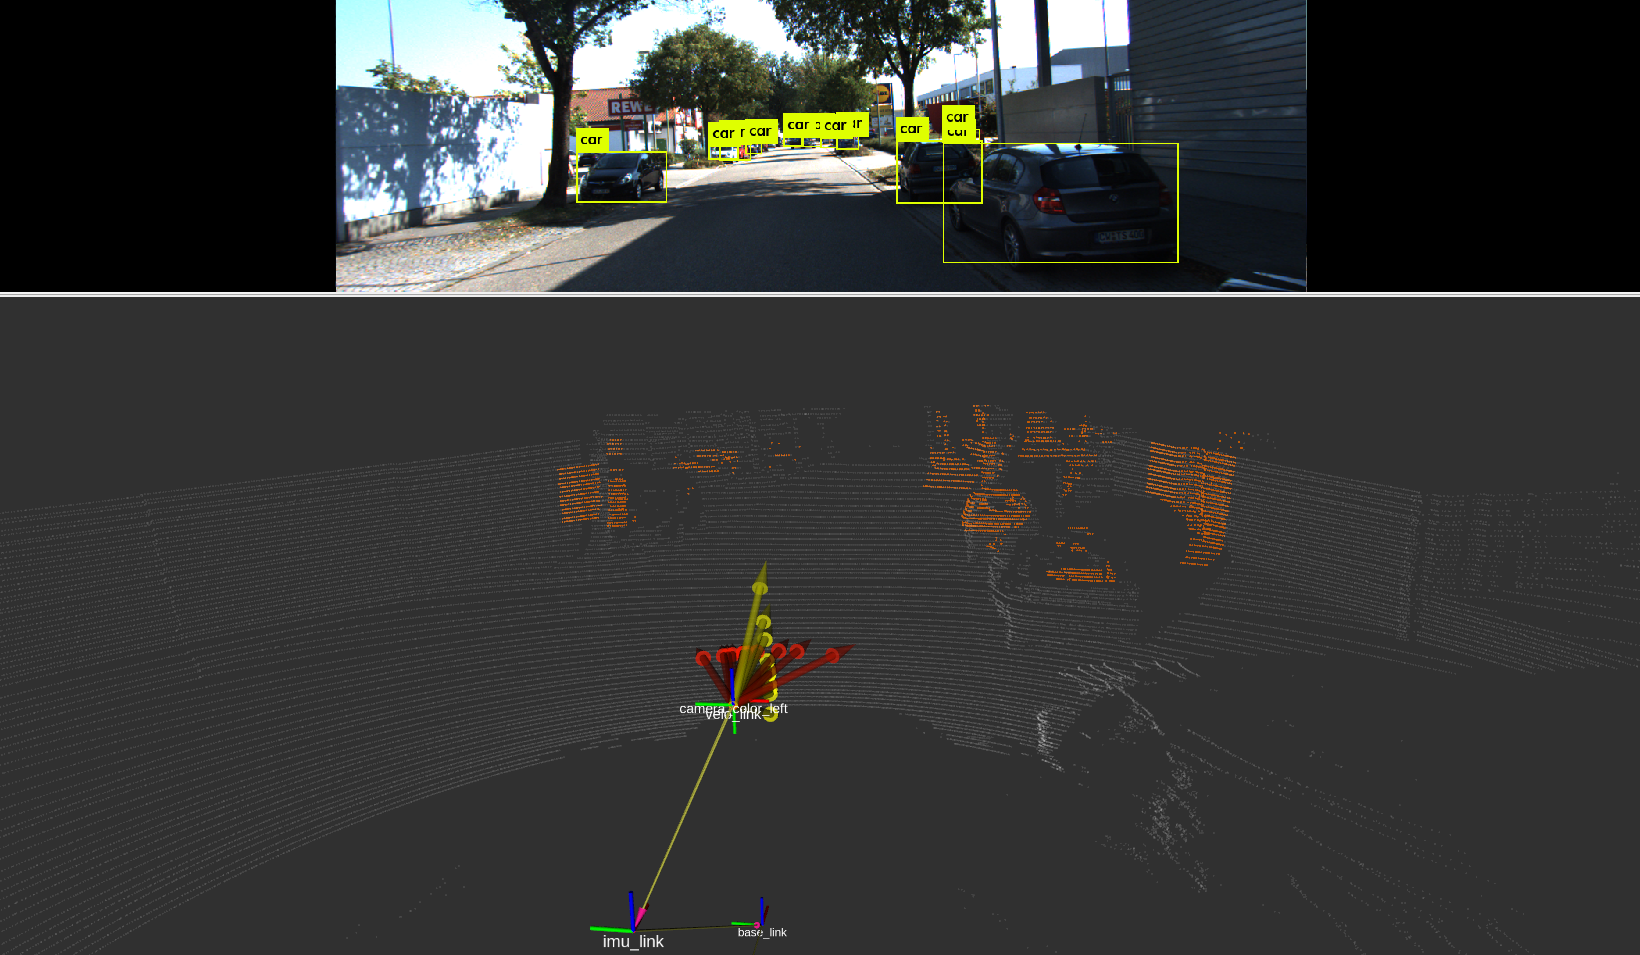
\includegraphics[width=0.8\textwidth]{img/image-object-to-point-cloud/bbox_correspondences_on_kitti.png}
	\caption{img/image-object-to-point-cloud/bbg}
	\label{fig:bbox-correspondences-on-kitti}
\end{figure}

The results are not as expected, as one can easily see that the filtered point cloud points (in orange) do not correspond to the objects on the image above. The code was debugged but the cause of the mismatch was not found, therefore a another algorithm to match the bounding boxes was developed. 


\subsection{Projection \ac{lidar} points to the image}
The alternative method to establish correspondences is similar to the one used for Sensor Fusion, detailed in Chapter~\ref{chapter:sensor-fusion}. The difference between the implementation on the latter chapter and this is that instead of comparing if the projected \ac{lidar} points correspond to a pixel on the image, they must also be contained in a bounding box. 

Similar to the conversion on Chapter~\ref{chapter:sensor-fusion}, the coordinate conversion frame is the rigid body transform determined in section~\ref{sec:calibration:extrinsic}.

\subsubsection{Extract Indices}
For every match, the index of that point is register. Later the \ac{pcl} Extract Indices filter is used to create a new point cloud that contains only the points that correspond to an object of the point cloud.

\subsubsection{Implementation}
The implementation is based on the implementation detailed on section~\ref{chapter:object-detection:image}. A new node, responsible for extracting the indices is implemented, \texttt{correspondences\_finder}, publishing a filtered point cloud containing all the points that belong to the \acp{roi} correspondent to the image bounding boxes. The node diagram can be seen on figure~\ref{fig:correspondences-finder-standalone}.

\begin{figure}[H]
	\centering
	\def\svgwidth{\columnwidth}
	\graphicspath{{img/image-object-to-point-cloud/}}
	\includesvg{img/image-object-to-point-cloud/correspondences-finder-standalone}	
	\caption{Hello}
	\label{fig:correspondences-finder-standalone}
\end{figure}

\subsubsection{Results}
The filtered \acp{roi} from the original point cloud can be seen on figure~\ref{fig:projected-correspondences}.

\begin{figure}[H]
	\centering
	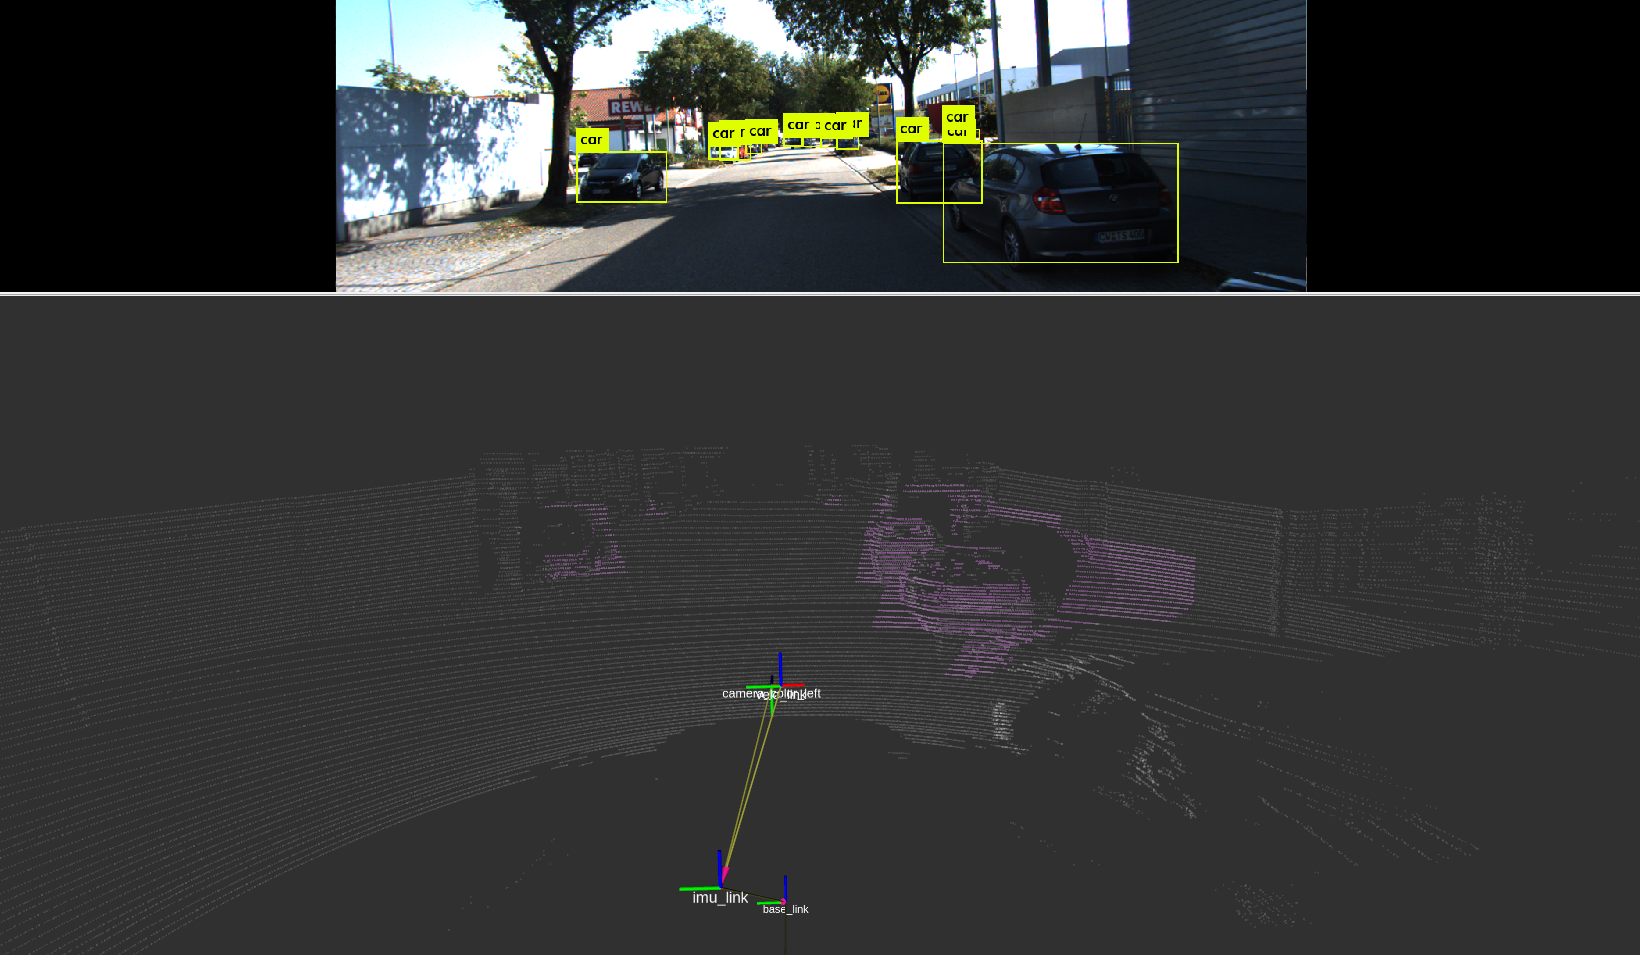
\includegraphics[width=0.8\textwidth]{img/image-object-to-point-cloud/projected_correspondences.png}
	\caption{img/image-object-to-point-cloud/prg}
	\label{fig:projected-correspondences}
\end{figure}

Comparing the results between the two approaches, on figure~\ref{fig:matching-comparison}, 

\begin{figure}[H]
	\centering
	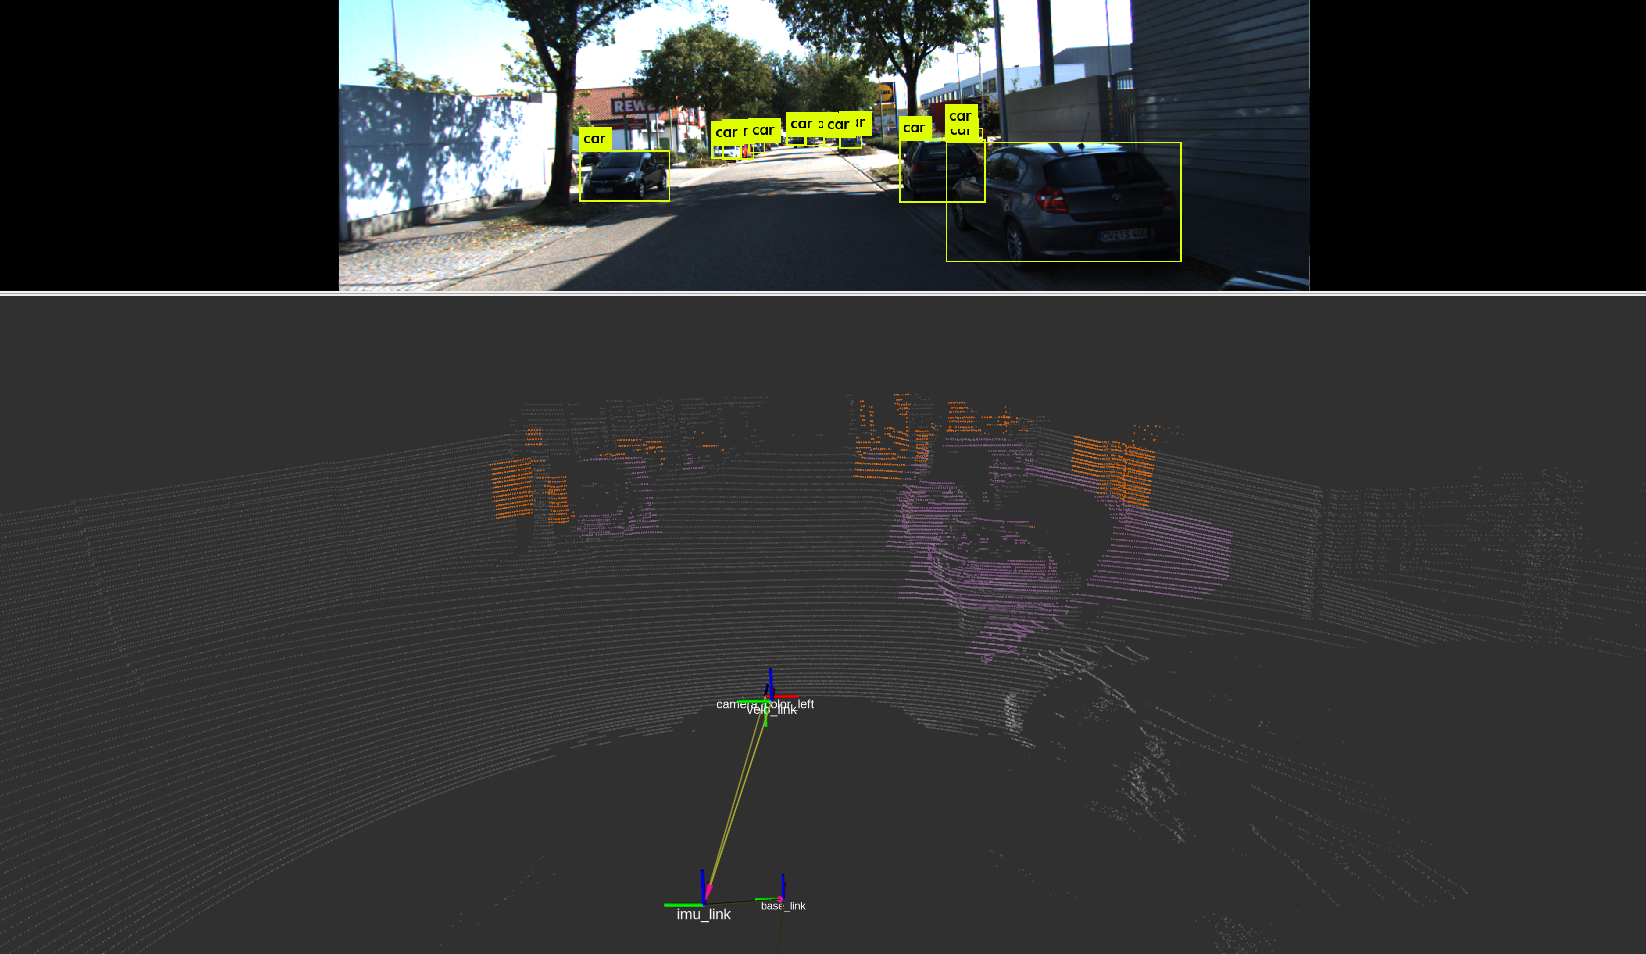
\includegraphics[width=0.8\textwidth]{img/image-object-to-point-cloud/rois-comparison.png}
	\caption{Matching Comparison between the two algorithms.}
	\label{fig:rois-matching-comparison}
\end{figure}

\subsection{3D Bounding Boxes and \aclp{roi}}

%Estimating a \ac{roi} on a point cloud from an image has the caveat of requiring the conversion between a 2D object (a rectangle representing a bouding box) to a 3D object (a parallelipedide representing a bounding box). As detailed on the Chapter~\ref{chapter:sensor-fusion}, such convertion requires the estimation of one degree of freedom whose information is not on the image: depth. However, on that chapter, the problem was solved by addressing it from another point opf view (projection of 3D points to an image and then coloring them). 

\subsubsection{Voxelization}

\subsubsection{Clustering}

\subsubsection{Bounding Box Estimation}

PCA
OBB
ABB

\section{Final Remarks}









